\section{Application in Agentic Tasks}
\label{sec:applications}

\subsection{Overview}

In this section, we investigate the potential of MemT-1.0 for developing self-evolving agents through continual learning. We apply MemT-1.0 to long-horizon agentic tasks, where agents must use environment feedback to guide task execution. Real-world agent interactions generate a wealth of trajectories containing valuable procedural experience. Reusing this experience offers a promising path toward improving agent performance across tasks. Current methods typically extract experience from historical trajectories and include it in the textual context of subsequent tasks~\cite{zhao2024expel}, increasing the burden on an already growing execution context. MemT-1.0 can instead store experience in native memory and use it to guide actions in long-horizon tasks.

We focus on agentic coding and train MemT-1.0-Nano to apply procedural experience extracted from historical trajectories. We evaluate it on SWE-bench Verified and SWE-bench Multilingual against Qwen3.6-35B-A3B, both without experience and with textual experience. With experience stored before execution, MemT-1.0-Nano improves the proportion of tasks solved in all three runs over the backbone without experience by 7.6 percentage points on SWE-bench Verified and 8.3 points on SWE-bench Multilingual. Results show that MemT-1.0 can improve agentic task performance beyond memory-focused evaluations and support its potential as a foundation for self-evolving agents.

\subsection{Experience-Guided Agentic Framework}
\label{sec:app-method}

To explore this potential, we develop an agentic framework in which MemT-1.0 stores and reuses procedural experience during long-horizon task execution.
We construct an experience bank by summarizing historical agent trajectories into reusable procedural guidance. As illustrated in Figure~\ref{fig:app-harness}, the framework retrieves relevant experience from the bank and stores it in either the agent's textual context or MemT-1.0-Nano's native memory. The two approaches use the same experience but differ in how it is accessed during task execution.

\textbf{Experience Retrieval and Storage.}
Given a coding task, we retrieve relevant experiences from the experience bank using BGE-M3~\cite{chen2024bgem3}. Each experience describes its applicable conditions, recommended procedures, and verification strategies. The task description serves as the retrieval query, and candidate experiences are ranked according to embedding similarity. The selected experience is converted into a structured textual representation before storage.

We consider two experience storage settings.
In the Before Execution setting, experience is stored before the agent begins execution. In the Harness-Triggered setting, the agent first executes the task independently, and experience is stored when the execution harness detects a critical breakpoint. Such breakpoints are identified using execution feedback, including command failures, empty observations, and repeated unsuccessful operations. The detection only relies on information available during execution, without accessing reference solutions. Each trajectory receives at most one experience store operation.

\textbf{Memory-Based Experience Application.}
In the Textual Experience setting, the retrieved experience is directly inserted into the agent's message history and remains available through the subsequent context. In the Native Memory setting, MemT-1.0-Nano writes the same experience into its native memory state through a separate memory store operation. Specifically, the experience text is processed by a forward pass with memory writing enabled, updating the memory state $M$ without modifying the original task context. After the memory store operation, agent actions access the stored experience through memory attention, allowing the experience to influence action generation without explicitly appearing in the message history.

Each execution trajectory maintains an independent memory state. The state is initialized to empty before the task and updated when experience is stored. After storing experience, it remains fixed and is read during subsequent execution until it is reset at the end of the trajectory. This setup evaluates whether a trained native-memory agent can effectively reuse procedural experience without retaining the experience text in the task context.

\begin{figure*}[t]
    \centering
    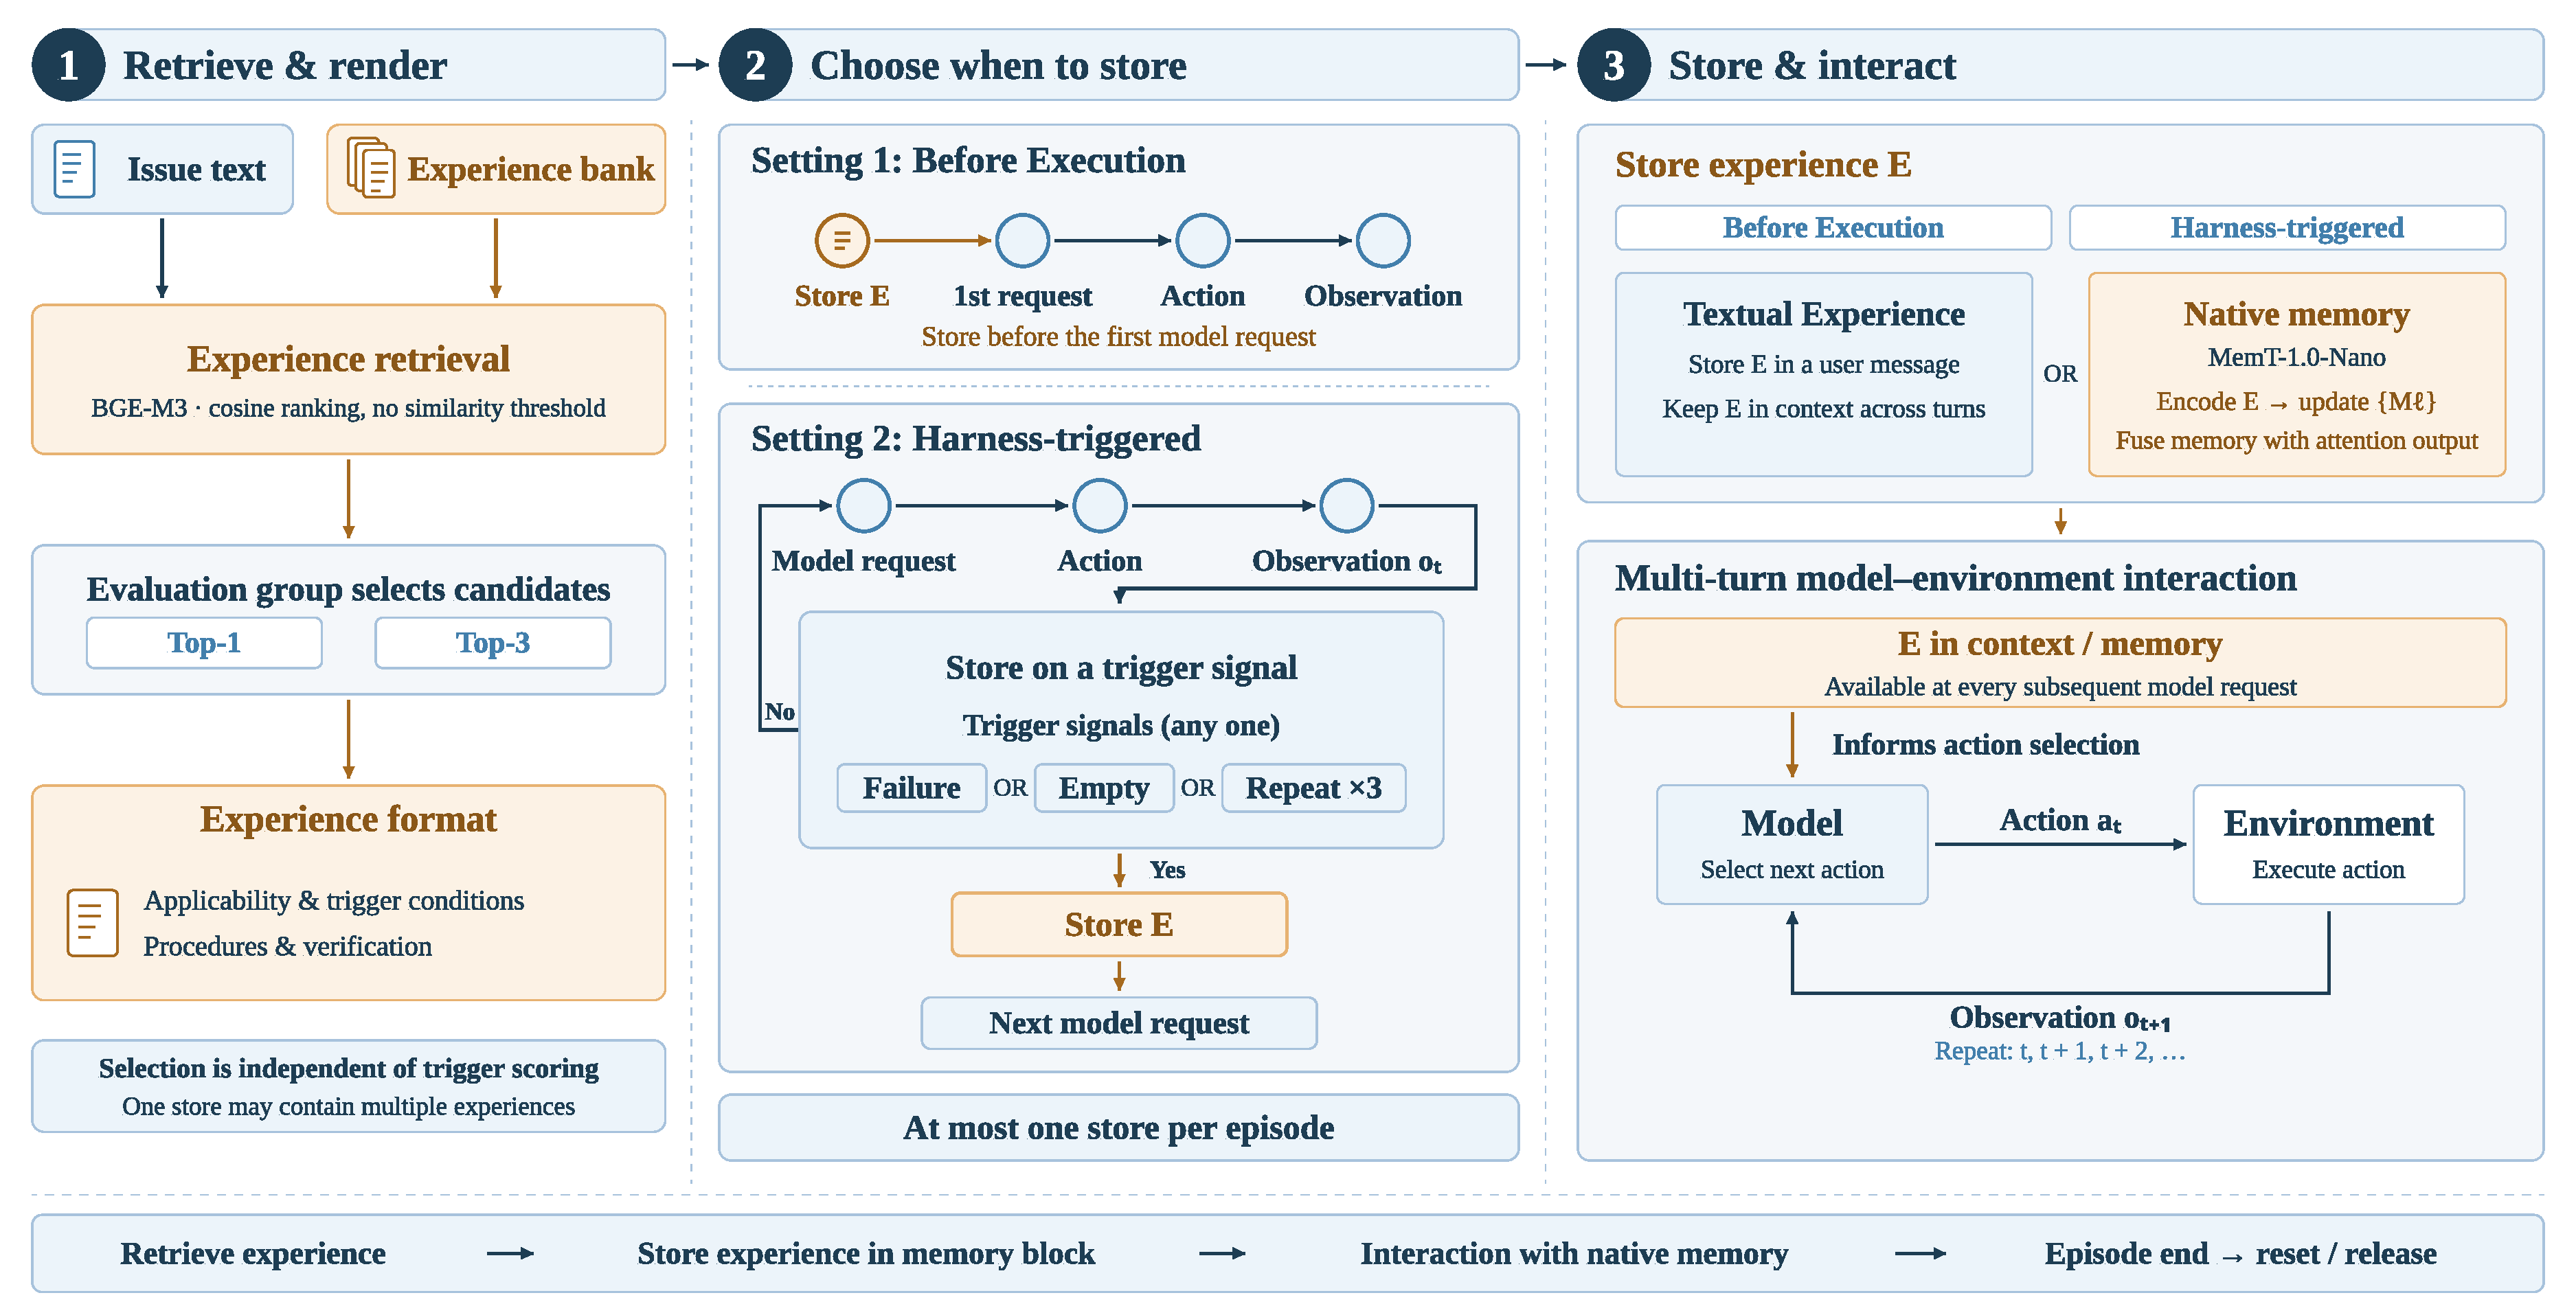
\includegraphics[
        width=0.95\textwidth
    ]{figures/application.pdf}
    \caption{
        Experience-guided agentic framework with MemT-1.0-Nano. Retrieved experience is stored in textual context or native memory to guide subsequent actions.
    }
    \vspace{-0.4cm}
    \label{fig:app-harness}
\end{figure*}


\subsection{Experience Construction and Model Training}
\label{sec:app-data-training}

To enable experience-guided agentic execution through native memory, we construct training data that associate reusable procedural experience with successful execution behaviors. The overall data construction consists of two stages, extracting reusable experience from historical trajectories and generating experience-conditioned trajectories.

\textbf{Experience Data Construction.}
We first construct an experience bank from 41,057 successful coding trajectories released by Scale-SWE~\cite{zhao2026scaleswe}. Following the experience summarization framework of MSCE~\cite{tang2026msce}, the construction process consists of trajectory annotation, procedural policy induction, policy clustering, and experience generation with quality auditing. For each successful trajectory, we identify important execution decisions and their corresponding environmental conditions. Trajectories with similar conditions are grouped to induce reusable procedural policies, which are subsequently consolidated and converted into structured experiences. Each experience contains information about its triggering conditions, recommended execution steps, applicability constraints, and verification procedures. After quality filtering, we obtain an experience bank containing 1,040 reusable coding experiences.

\textbf{Training Sample Construction.}
We further construct experience-guided training trajectories through counterfactual execution. Specifically, we generate original coding trajectories using Qwen3.6-35B-A3B with the AweAgent harness~\cite{aweagent2026} in the Scale-SWE environment. For unsuccessful trajectories, we identify candidate breakpoints according to execution errors and other observable failure signals. At each selected breakpoint, we retrieve candidate experiences and resume execution with different experience combinations. The resulting trajectories are evaluated using executable tests, and we retain experience-conditioned continuations that pass the task tests when the corresponding original trajectory failed.

Each training sample is represented as
\begin{equation*}
    x_{b,j} =
    \left(
        \xi_{\leq b},
        g_{b,j},
        \hat{\xi}_{>b}^{+}
    \right),
\end{equation*}
where $b$ indexes the selected breakpoint and $j$ indexes the candidate experience subset. Here, $\xi_{\leq b}$ denotes the original trajectory prefix before and including breakpoint $b$, $g_{b,j}$ denotes the injected experience subset, and $\hat{\xi}_{>b}^{+}$ denotes the successful continuation after experience injection. 


The retained samples satisfy the condition that the original trajectory fails while the experience-conditioned continuation succeeds. These continuations provide supervision for predicting successful actions conditioned on procedural experience. We generate 18,820 original trajectories and evaluate 199,500 breakpoint-experience intervention variants. Among these interventions, 45,481 produce successful continuations. After additional quality filtering, we obtain 42,403 training samples. The resulting samples are partitioned by task to avoid leakage between training and validation trajectories. Appendix~\ref{appendix:detail_application} provides details of the experience bank, data construction pipeline, and filtering procedure.


\textbf{Training Strategy.}
We initialize the model from MemT-1.0-Nano. During application-specific post-training, all backbone parameters are frozen, and only the native hyper memory blocks are optimized. Each training sample is processed through separate experience and main-trajectory streams. First, the experience is written into native memory through a memory store operation. The original trajectory prefix is then replayed with memory reading disabled. After the designated breakpoint, memory reading is enabled, and the model is trained to predict the successful continuation conditioned on the stored experience. The experience text and trajectory prefix are excluded from the training loss, while the subsequent assistant actions provide the supervision signal.

We investigate both cross-entropy supervision and knowledge distillation. For knowledge distillation, the frozen backbone teacher receives the experience as text, while the student accesses the same experience only through native memory. Both models use teacher forcing on the same task history and reference continuation. We minimize the forward KL divergence from the teacher distribution to the student distribution over supervised assistant tokens.

We additionally investigate two supervision scopes.
The First-Step setting supervises only the first assistant turn following the breakpoint, and the Full-Suffix setting supervises the complete successful continuation. We use knowledge distillation with Full-Suffix supervision for the application-specific post-training of MemT-1.0-Nano and evaluate the resulting checkpoint in the main experiments. Appendix~\ref{appendix:detail_application} details the sample serialization and supervision masks.

\subsection{Agentic Coding Evaluation}
\label{sec:app-evaluation}

We evaluate MemT-1.0-Nano on two agentic coding benchmarks, including SWE-bench Verified~\cite{chowdhury2024swebenchverified}, containing 500 tasks, and SWE-bench Multilingual~\cite{Yang2025SWEsmithSD}, containing 300 tasks across nine programming languages. Both benchmarks require agents to resolve real-world software issues through repository exploration, code modifications, and executable tests. All baselines use Qwen3.6-35B-A3B as the backbone and follow the official SWE-bench verification protocol.

We compare Qwen3.6-35B-A3B (No Experience), Qwen3.6-35B-A3B (Textual Experience), and MemT-1.0-Nano (Native Memory). The \textbf{No Experience baseline} measures the benefit of experience reuse, while \textbf{Textual Experience} provides a reference for evaluating its effectiveness through native memory. The Harness-Triggered setting uses the same breakpoint-detection logic as training data construction. The Before Execution setting is used to assess robustness to experience injection timing. Each task is executed three times independently.

As shown in Table~\ref{tab:app-main-results}, we report the average success rate, \texttt{pass@3}, representing the proportion of tasks solved at least once across the three runs, and \texttt{pass\textasciicircum{}3}, representing the proportion of tasks solved in all three runs.
\textbf{MemT-1.0-Nano consistently improves the average success rate and repeated-run reliability over the backbone without experience.} On SWE-bench Verified, in the Before Execution setting, MemT-1.0-Nano achieves an average success rate of 69.33\%, improving upon the No Experience baseline of 66.07\%. This slightly exceeds the 68.87\% achieved by Textual Experience. Moreover, \texttt{pass\textasciicircum{}3} increases from 54.00\% to 61.60\%, matching the 61.60\% achieved by Textual Experience. These results indicate that \textbf{native memory can preserve the effectiveness of procedural experience without requiring the corresponding experience text to remain in the task context}.



\begin{table*}[t]
    \centering
    \caption{
        Agentic coding performance on SWE-bench Verified (500 tasks) and SWE-bench Multilingual (300 tasks) under two experience injection settings.
        Bold and underlined values indicate the highest and
        second-highest distinct scores, respectively.
    }
    \label{tab:app-main-results}
    \vspace{-0.1cm}

    \small
    \setlength{\tabcolsep}{5pt}
    \renewcommand{\arraystretch}{1.16}

    \sisetup{
        detect-weight = true,
        detect-family = true,
        round-mode = places,
        round-precision = 2,
        round-pad = true,
        table-alignment-mode = none,
        table-number-alignment = center,
        table-text-alignment = center
    }

    % First and second place
    \newcommand{\appfirst}[1]{%
        \multicolumn{1}{c}{\textbf{#1}}%
    }
    \newcommand{\appsecond}[1]{%
        \multicolumn{1}{c}{\underline{#1}}%
    }

    \newcolumntype{Y}{
        S[
            table-format = 2.2,
            table-fixed-width = true,
            table-column-width = 5.5em,
            table-alignment-mode = none,
            table-number-alignment = center
        ]
    }

    % Scale the table and its notes together.
    \begin{adjustbox}{max width=\textwidth}
    \begin{threeparttable}

    \begin{tabular}{
        l
        l
        l
        Y Y Y
    }
        \toprule

        \rowcolor{MetisBlueDark}
        \color{white}\bfseries Benchmark
        & \color{white}\bfseries Store Timing
        & \color{white}\bfseries Method
        & \multicolumn{1}{c}{\color{white}\bfseries
            \mbox{pass\textasciicircum{}3}}
        & \multicolumn{1}{c}{\color{white}\bfseries Avg. Success}
        & \multicolumn{1}{c}{\color{white}\bfseries pass@3} \\

        \midrule

        % ===== SWE-bench Verified =====

        \multirow{6}{*}{Verified}
        & \multirow{3}{*}{Before Execution}
        & Qwen3.6-35B-A3B (No Experience)
        & \appsecond{54.00}
        & 66.07
        & \appfirst{77.60} \\

        & & Qwen3.6-35B-A3B (Textual Experience)
        & \appfirst{61.60}
        & \appsecond{68.87}
        & 76.40 \\

        & & \textbf{MemT-1.0-Nano (Native Memory)}
        & \appfirst{61.60}
        & \appfirst{69.33}
        & \appsecond{77.40} \\

        \cmidrule(lr){2-6}

        & \multirow{3}{*}{Harness-Triggered}
        & Qwen3.6-35B-A3B (No Experience)
        & 54.00
        & 66.07
        & \appsecond{77.60} \\

        & & Qwen3.6-35B-A3B (Textual Experience)
        & \appsecond{61.80}
        & \appsecond{69.13}
        & 76.80 \\

        & & \textbf{MemT-1.0-Nano (Native Memory)}
        & \appfirst{62.80}
        & \appfirst{69.73}
        & \appfirst{77.80} \\

        \midrule

        % ===== SWE-bench Multilingual =====

        \multirow{6}{*}{Multilingual}
        & \multirow{3}{*}{Before Execution}
        & Qwen3.6-35B-A3B (No Experience)
        & 45.33
        & 60.00
        & \appfirst{73.67} \\

        & & Qwen3.6-35B-A3B (Textual Experience)
        & \appfirst{56.33}
        & \appfirst{64.22}
        & \appsecond{72.67} \\

        & & \textbf{MemT-1.0-Nano (Native Memory)}
        & \appsecond{53.67}
        & \appsecond{62.89}
        & 72.00 \\

        \cmidrule(lr){2-6}

        & \multirow{3}{*}{Harness-Triggered}
        & Qwen3.6-35B-A3B (No Experience)
        & 45.33
        & 60.00
        & \appfirst{73.67} \\

        & & Qwen3.6-35B-A3B (Textual Experience)
        & \appsecond{53.67}
        & \appsecond{63.00}
        & 72.67 \\

        & & \textbf{MemT-1.0-Nano (Native Memory)}
        & \appfirst{55.33}
        & \appfirst{63.56}
        & \appsecond{73.00} \\

        \bottomrule
    \end{tabular}

    \begin{tablenotes}[flushleft]
        \footnotesize
        \item[]
        All values are percentages, based on three
        independent runs per task.
        The \mbox{pass\textasciicircum{}3} denotes the percentage of tasks solved in all three runs.
        The Avg. Success denotes the mean success rate across runs.
        The pass@3 denotes the percentage of tasks solved in at
        least one run.
        % \item[]
        Textual Experience uses the top 3 experiences for Verified Before Execution; top 1 otherwise.
    \end{tablenotes}

    \end{threeparttable}
    \end{adjustbox}

    \vspace{-0.4cm}
\end{table*}



In the Harness-Triggered setting, MemT-1.0-Nano further improves the average success rate to 69.73\%, compared with 66.07\% for No Experience and 69.13\% for rank-1 textual experience. The corresponding \texttt{pass\textasciicircum{}3} reaches 62.80\%, representing an improvement of 8.80 percentage points over the backbone and 1.00 percentage point over fixed rank-1 textual experience. This suggests that native memory remains effective when experience is introduced dynamically during agent execution, rather than only at task initialization.

We observe consistent improvements on SWE-bench Multilingual. In the Before Execution setting, MemT-1.0-Nano improves the average success rate from 60.00\% to 62.89\% and \texttt{pass\textasciicircum{}3} from 45.33\% to 53.67\%. In the Harness-Triggered setting, the average success rate reaches 63.56\%, exceeding the fixed rank-1 textual experience result of 63.00\%. These findings provide further evidence that experience internalization generalizes across coding tasks involving different repositories and programming languages.

The gains are most pronounced in repeated-run reliability, suggesting that stored experience helps agents solve tasks more consistently. Although \texttt{pass\textasciicircum{}3} improves substantially, \texttt{pass@3} does not consistently increase.
The comparable behavior of MemT-1.0-Nano and textual experience further suggests that procedural guidance can be represented and utilized through native memory.


We also evaluate several training configurations on a 100-task development subset of SWE-bench Verified. Detailed comparisons and additional experimental results are provided in Appendix~\ref{appendix:detail_application}.


\subsection{Case Study and Discussion}
\label{sec:app-discussion}

To better understand how native memory affects agent behavior, we illustrate a representative task from SWE-bench Verified involving the two-digit year parsing logic in Django's \texttt{parse\_http\_date} function. 

We compare execution trajectories under the No Experience, Textual Experience, and Native Memory settings. Without experience, the agent modifies the relevant parsing logic shortly after locating the implementation, introducing targeted reproduction and verification steps later in the execution. In contrast, agents in both the Textual Experience and Native Memory settings construct reproduction tests before applying modifications. In the MemT-1.0-Nano trajectory, the agent further revisits a boundary condition after its initial modification, corrects the implementation, and performs additional verification.

These observations show how stored procedural experience can guide task execution without appearing in textual context. Together with the benchmark improvements, they demonstrate that MemT-1.0 can reuse procedural experience to improve agentic task performance. This supports its potential for developing self-evolving agents: \textbf{experience from past interactions can be stored in native memory and applied to new tasks.}

Several challenges remain. The current framework relies on externally constructed experience, making its effectiveness dependent on experience quality and retrieval. Storing experience also introduces computation, so reduced textual context does not necessarily imply lower overall execution costs. Extending experience reuse into an autonomous continual learning process remains an open direction.

Future work will explore the co-evolution of the harness and MemT-1.0 through continued interaction with the environment. The harness can improve experience acquisition and selection, while MemT-1.0 learns to reuse that experience more effectively. Together, these advances could support continual learning in self-evolving agents for long-horizon tasks.
